\chapter{Background} \label{chap:backAndPb} %and Problem description
\begin{bibunit}[ieeetr]
\minitoc
\vspace{2cm}
%
\noindent
\begin{minipage}[c]{0.3\textwidth}
\centering
\includegraphics[width=\textwidth]{carsharing}\\
~\\
\includegraphics[width=.7\textwidth]{cube2}
\end{minipage}
\hfill
\begin{minipage}[c]{0.7\textwidth}
\begin{abstract}
%This chapter introduces the background interest of this thesis.
%Carsharing systems and their characteristics are fist described and their legitimacy as an interesting solution to transportation issues is first highlighted.
%
%The chapter follows with the demand estimation problem.
%Assumptions made in this thesis and the approach we considered are exhibited.
%
%Finally, the chapter concludes with a focus on the problem addressed in this manuscript.
\end{abstract}
\end{minipage}

\newpage
\section{Carsharing systems} \label{sec:carsharingSystems}

% a mettre en intro
% $>$ Why sharing is a good solution ?
% Recent mobility surveys highlight a decline in the use of private vehicles.
% The number of daily trip by car is decreasing in urban areas.
% Vehicle sharing systems, as bike sharing or carsharing systems, are now more and more widespread and popular in dense urban cities.
\subsection{Principles and brief history}
The main idea of carsharing is to share a fleet of cars between users.
Basically, it's a model of car rental where people rent cars for short periods of time.
Carsharing systems are mainly intended for occasional drivers whom gain the benefit of private vehicle use without the costs and responsibilities of ownership \cite{shaheen_carsharing_1998}.
Its principle is based on the vehicle usage rather than vehicle possession.
Costs related to insurance, maintenance, fuel (or electricity), taxes, depreciation, etc. are supported by car owners, \ie mostly cooperative organizations or private operators.
They differ and have to be distinguished from traditional auto-rental services mainly because they are oriented to short-term rentals and fuel costs are included in the rental fee.
Mainly located in dense urban areas, they contribute to fill the gap between existing modes of transportation \cite{louvet_enquete_2013}.

\medskip
Nowadays, there are many implementations of carsharing systems adopting many different forms but generally, individuals access vehicles on an as-needed basis by joining an organisation that maintains a fleet of vehicles (essentially cars and light trucks) in a network of locations.
These are usually deploy in the vicinity of public transport stations, neighbourhoods, employment centres and universities \cite{shaheen_carsharing_1998}.

\bigskip
Although the concept of carsharing is constantly evolving, one of the most concise definition could be the one given by Millard-Ball et al. in (2005) \cite{millard_ball_car_sharing_2005} which defines carshaing as
\begin{quote} % there are plenty of formal definition in the literature
``a membership program intended to offer an alternative to car ownership under which persons or entities that become members are permitted to use vehicles from a fleet on an hourly basis.''
\end{quote}
More recently, in 2010, the french law defined carsharing systems under these terms \cite{cs_loi_2010}:
\begin{quote}
``Carsharing is the pooling of an inland transport motor vehicles fleet for the benefit of subscribers. Each one of them can access a driverless vehicle for the ride of his choice for a limited time.''
\end{quote}

\bigskip
The first experiment of carsharing is identified in \cite{shaheen_short_1999} as Sefage, a Swiss company created in 1948.
For a variety of reasons, almost all effort at organising carsharing organisations resulted in failure until the early 1990's.
Different causes has been discussed to explain the origins of these common failures.
The list includes excessive financial costs, low demand, service quality deterioration, technological limitations, as well as a restricted service area and a lack of government support \cite{harms_emergence_1998, cousins_theory_2000}.

\medskip
Since then, many schemes of the system have been implemented and the basic concept of carsharing has evolved in many ways.
Over time, profit-making organisations have emerged as the most important actors in the carsharing market, even though the number of non-commercial and cooperative organisations is still the largest.
Lessons learned from unfortunate experiences combined with technological advances helped launching new carsharing programs.
Historically, first successful systems started in Europe.
Their development has highly contributed to spread and confirm the viability of vehicle-sharing systems across the world.
Today, the actual world's leader carsharing company is Zipcar.
Founded in 2000, its global vehicle fleet exceeds $12,000$ vehicles and $950,000$ members, mainly in the US \cite{zipcar_website}.

\medskip
Last decade has recorded the highest carsharing market growth.
In 2007, the total worldwide number of carsharing members was estimated to $348,000$ and the shared fleet of vehicles to nearly $11,700$ \cite{shaheen_growth_2007}.
Almost ten years later, in 2014, these numbers are approximated to $4,94$ millions ($\simeq \times 14$) and $92,200$ vehicles respectively ($\simeq \times 8$) \cite{statista_carsharingNumbers}.
Numerous programs are launched here and there among all continents.
It continues to expand in large part due to advanced technologies whose the greatest representatives are surely smart-phones.
Besides, incentive public policies allows private firms to reserve public on-street parking making the service more convenient and attractive.
Propitious indicators and worldwide experts anticipate further development for the forthcoming years \cite{shaheen_carsharing_2013}.

%%%%%%%%%%%%%%%%%%%%%%%%%
% a suivre : les types de carsharing et l'impact sur la société


% If the organisation renting the fleet may be , most of them are today run by a company managing the system. % a reformuler
% , as peer-to-peer carsharing for instance,

% (présentation CS)



\subsection{Carsharing models}
In this thesis, we focus on carsharing systems managed by private operators.
Three different models called respectively 'Round-trip', 'One-way' and 'Free-floating' can be find around the world.
They can be distinguished by their constraints related to the use of vehicles and the fact of having or not stations.
In order to access the service, carsharing companies generally required members to pay a yearly registration fees.
Sometimes it is a deposit that is refunded when membership ends.
Then, a monthly rate based on the time spent on roads and the distance travelled testifies to the personal usage of each member.

\medskip
The technology provided by the operator can vary enormously.
In Europe, most operator offer different kind of vehicles, from small city cars to large cargo vehicles.
Generally, members have access to vehicles on-the-go using smart cards or PIN (personal identification number).
They can also make a reservation online or using (smart)phones to guarantee the availability of a vehicle.
The service can sometimes be related to public transport, offering a large mobility supply to individuals.

\medskip
Round-trip and one-way systems are said \textit{station-based}.
They involve a small to medium fleet of vehicles, available at several stations, to be used by a relatively large group of members \cite{shaheen_short_1999}.
Vehicles are dispersed all across the city through many indicated stations, where a fixed number of parking places stores the vehicles.
Generally, carsharing companies dispose of their own dedicated parking lots situated on-street or off-street according to contractual arrangement with the entity (private or public) managing the parking.
The number of lots can varies according to the size of the system and the available urban space, but since carsharing is mainly implanted in dense urban areas, stations are often small.
In Paris, for instance, the number of parking places is between $4$ and $7$ \cite{autolib_rapport_2014}.
Also, station-based systems can provide additional specific infrastructure if necessary.
The carsharing service Autolib' in Paris, offers charging points for electric vehicles and kiosks for customer service.


\subsubsection{The Round-Trip system}
\begin{wrapfigure}[6]{r}{3cm}
\vspace{-.4cm}
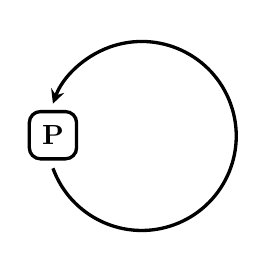
\begin{tikzpicture}[scale = .6]
\draw[very thick, rounded corners] (-.5,-.5) rectangle(.5,.5);
\draw node at (0,0){\textbf{P}};
%\fill[black] (0,0) circle (.5);
\draw[very thick, ->, > = stealth,] (0,-.7) arc (-160:160:2);
\end{tikzpicture}
\end{wrapfigure}
Historically, the first carsharing scheme to be implemented was the round-trip system.
As such, it is today the best established commercially and has been largely studied.
Basically, It requires users to return vehicles to the station they were picked up.
Such systems are simple to design since the incoming demand in each station is sufficient to plan vehicle stocks.
The user behaviour is mainly oriented to leisure and household shopping purpose \cite{barth_shared_use_2002, costain_synopsis_2012}.


\subsubsection{The One-way system}

\begin{wrapfigure}[6]{l}{3cm}
\vspace{-.4cm}
\centering
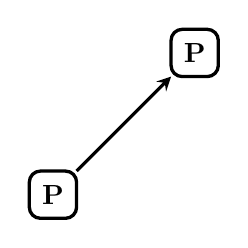
\begin{tikzpicture}[scale = .6]
\draw[very thick, rounded corners] (-.5,-.5) rectangle(.5,.5);
\draw node at (0,0){\textbf{P}};
\draw[very thick, rounded corners] (2.5,2.5) rectangle(3.5,3.5);
\draw node at (3,3){\textbf{P}};
%\fill[black] (0,0) circle (.5);
%\fill[black] (3,3) circle (.5);
\draw (.5,.5) edge[very thick, ->, > = stealth,] (2.5,2.5);
\end{tikzpicture}
\end{wrapfigure}

One-way carsharing scheme is more flexible than round-trip.
It allows users to pick up a vehicle from a station and return it in a different one, possibly distinct from the origin.
Unfortunately, this greater flexibility comes with hard operational problems due to the uneven nature of the trip pattern in urban areas.
Indeed, empty stations exclude potential requests to be satisfied.
Conversely, crowded stations do not allow an incoming vehicle to park.
Thus, the system imbalance must be corrected so that vehicles can be relocated to suitable places.
This problem referred as the vehicle imbalance problem is discussed thereafter.
%, listed and described below,

However, let notice that despite these difficulties for the operator, one-way system captures more trips than the alternative system thanks to this flexibility which is a critical factor to join a carsharing scheme \cite{efthymiou_which_2012}.


\subsubsection{The Free-floating system}

\begin{wrapfigure}[6]{r}{3cm}
\vspace{-.4cm}
\centering

\begin{tikzpicture}[scale = .6, > = stealth,]
\fill[black] (0,0) circle (.5);
\foreach \angle in {0,45,...,315} {
\draw (\angle:0.6) edge[very thick, ->, > = stealth,] (\angle:2);
};
\end{tikzpicture}
\end{wrapfigure}

Nowadays, many carsharing schemes have been tested and experimented.
Although first ones have been station-based designed, we have witnessed in the last decade the emergence of carsharing models without stations.
The user can picked up on-street parked vehicles owned by the system operator and parked on any legal parking space within a defined area.
This new feature comes with the propensity to assign more and more flexibility to the service.
Point-to-point free-floating carsharing (often referred to as flexible carsharing) corresponds to a sharing scheme where usage is typically spontaneous.
Vehicle reservations are mostly made several minutes in advance.
The system operator ensures a service quality based on vehicle maintenance and available parking places.
The largest free-floating system is operate by car2go mainly in Germany.
In 2015, the service account for more than one million members.
% whereas the third one, appeared recently, offers more flexibility 

\subsection{Positive impacts}
% on the transportation system
As an innovative alternative to private car ownership, carsharing is a interesting trade off between distance and flexibility.
On the one hand, the car provides the freedom to cover entire urban areas.
Even with electric vehicles, for which the autonomy is limited, distances of more than $150$ kilometres can be considered.
On the other hand, the fact that cars are available on-demand relieves users from the rigidity of public transport timetables.
Moreover, station-based carsharing systems aim at reducing the time spent at searching for a parking lot, which is often important in dense urban areas.
In France, its contribution to the global congestion is evaluated between $5$ and $10$\%  \cite{stationnement_intelligent_cerema}.
As a consequence, carsharing is now considered as an attractive transportation mode filling the gap between traditional public transport and private vehicle use.

\medskip
In the last decade, several authors have showed that carsharing systems have positive impacts on users, the transportation system and the environment.
Although not all of these commonly attested benefits are documented with empirical data, next sections present substantial agreements about carsharing on the urban mobility, financial gains and the environment.


\subsubsection{Urban mobility}

The carsharing economic model is founded on the use of the vehicles.
The cost for moving from A to B depends on the distance and the time the user spend on the road.
As such, carsharing infers on user behaviours, whom aligned their car usage on those criterion, and consequently provides greater incentive for members to be selective about driving.

% inherent
% infer
A study conducted in 2004 reports that carsharing users reduce their vehicle kilometres traveled (VKT) - or vehicle miles traveled (VMT) - by $50$\% after joining the organisation \cite{cervero_city_2004}.
More recent result evaluated this decrease to $27$\% in 2011 \cite{martin_greenhouse_2011}.

% Besides, some surveys indicate that carsharing users tend to optimize their trips more often than with their own car.

Besides, the use of carsharing systems led to a fall in car ownership rates and lower car use.
The number of vehicles per household is half lower for carsharing users \cite{martin_impact_2010, ter_schure_cumulative_2012}.

Moreover, the 


 shared vehicles spend more time on the road and less time parked (which represent for a private car almost 95\% of its total use time, as mentioned in \cite{transflash_2013})
Sharing a vehicle allows members to share its cost.




It also decreases the total number of vehicles on the road, since one vehicle can be driven by several users and thus improving the traffic fluidity.




As a consequence, parking requirements in dense areas decreases \cite{mitchell_reinventing_2010} as well as the average number of vehicles per household \cite{martin_impact_2010, ter_schure_cumulative_2012}.

Because of higher utilization rates than private vehicles \cite{litman_evaluating_2000, schuster_assessing_2005}, many studies show that using carsharing help decrease the number of vehicles on the road.

\subsubsection{Economical aspects}
General costs related to car ownership are commonly split into fixed and variable expenses.
According to the total distance travelled, driving habits or local parking costs, the variable costs might be very different from one car owner to the other.
However, the share of fixed costs, such as the purchase price of the vehicle, its depreciation over time or insurance, still remains predominant \cite{cout_reel_auto}.
In this context, embracing a carhsharing service where the price only depends on the vehicle usage can grants its users the car mobility at interesting costs.

\medskip
Nevertheless, those benefits are not relevant for every car user.
Basically, the less the car is used, the more carsharing services become interesting.
With respect to local costs, researches have shown that only car users driving less than $10,000$ kilometres per year (as much as \hbox{$15,000$ km/y}) could save money using carsharing \cite{litman_evaluating_2000, prettenthaler_ownership_1999}.

% using carsharing is considered as a complementary affordable mobility solution that may replace the car ownership for some individuals.

% Different studies evaluated that carsharing could be a real alternative to private car.


\subsubsection{Environmental effects}
Furthermore, it is now recognized that carsharing systems have positive environmental effects.
It reduces greenhouse gas (GHG) and CO2 emissions \cite{martin_greenhouse_2011, firnkorn_what_2011} and provides noise reduction since electric cars are quitter than thermal ones.
In addition, the reduction of parking demand can be used to reallocate the land for additional green spaces, new mixed-use development, or other community needs \cite{cohen_carsharing_2008}.


%As we explain below, these results are very important to calibrate simulation tools and have a good estimation of the demand.

%Because of their greater scientific interest compared to the ``round-trip'' carsharing system, we will now focus on the ``one-way'' carsharing system and develop more explicitly the main research areas and their main outcomes.

\subsection{Related problems}

\cite{leclerc_unraveling_2013} (comportement des utilisateurs carsharing)\\

\subsubsection{Demand estimation}
Some studies are also conducted to characterize and analyse who the users of these systems are.
Using statistical data and surveys, most studies demonstrated important tendencies: high correlation with the use of public transports, dwelling place in dense areas \cite{cervero_city_2003, millard_ball_car_sharing_2005, burkhardt_who_2006}, age between mid-30s to mid-40s, people highly educated and environmentally aware \cite{costain_synopsis_2012, efthymiou_which_2012, millard_ball_car_sharing_2005, brook_carsharingstart_2004, lane_phillycarshare_2005, zheng_carsharing_2009}.
Moreover, as showed in \cite{costain_synopsis_2012, efthymiou_which_2012, zheng_carsharing_2009}, the accessibility to the stations, in terms of distance between home/work and the nearest station, is a critical factor to joining a carsharing system.

\medskip
To be able to give a good prediction of a carsharing service, it's really important to identify the main factors which generate and influence the demand.
Stillwater et al. \cite{stillwater_carsharing_2009} have concluded that the most significant variables were: the street width (-), the provision of a railway service (-), the percentage of drive-alone commuters (-), the percentage of households with one vehicle (+), and the average age of the stations (+).
We indicate by (-) or (+) when the indicator is negatively or positively related to carsharing demand.
The street width and the percentage of drive-alone commuters may not have a clear intuitive explanation at first sight although those metrics are significantly related to the level of carsharing demand.
The authors postulate that street width contains informations about pedestrian environment (where narrow streets are more pedestrian friendly) and about the land use in general (narrow streets trend to denote older residential or mixed-use development) witch make sense since carsharing and walking behaviour are known (see e.g. \cite{cervero_city_2003}) to be strongly related.
The proportion of drive-alone commuters are negatively related because these people generally would already own vehicles and high level of vehicle commuting tend to signify a neighbourhood that has poor public transit or other high-density mode amenities.

\medskip
Another study conducted by Ciari et al. \cite{ciari_estimation_2013} uses an activity-based micro-simulation model to estimate travel demand and understand the effect carsharing system on urban mobility, considering others transportation modes such as public transport, car, bicycle and walking.
They suggested and evaluated a cost function in an open-source activity-based multi-agent simulator called MATSim \cite{matsim_webPage} which informs the user of the cost using carsharing as mode of transportation.
Thus, they have led to a modal split model, giving plausible results compared to real data (the urban area of Zurich, Switzerland), which can capture the proportion of total demand that could use this mode of transportation, depending on the access to the cars and the dependent fee structure.
In most cases, studies are context specific.
Trip patterns and travel behaviour can be different from one country to another since it is related to local and regional characteristics (culture, habits, etc.), making the standardization more complex.
Furthermore, as mentioned in \cite{jorge_carsharing_2013}, demand estimation has not so far been addressed in the literature for one-way carsharing systems, and a relevant model for such models is nowadays not available.
This is a real challenge for the future since it's reasonable to think that one-way carsharing systems will be increasingly present in the coming years.

\subsubsection{The vehicle imbalance problem}
As said before, the most challenged carsharing system is the one-way system. Since the arrival station is not necessary the same than the departure station in those systems, it induces and generates imbalance issues.
Thereby, a lot of efforts are made to understand the dynamics and find possible solutions to handle it.
The intuitive approach for solving the vehicle imbalance problem is to consider that the operator have to do periodic relocation operations among stations.
Some studies, using discrete event simulation models (see for example \cite{barth_simulation_1999, kek_relocation_2006, kek_decision_2009}), help operators to manage their systems minimizing available resources (such as vehicles and staff members), while maintaining certain levels of service.
The model presented in \cite{kek_decision_2009} has been tested and validated using real data (a one-way carsharing system called Honda ICVS) and proposed solutions reducing staff cost of about 50\%.

\medskip
Other authors have explored the problem under the optimization methods perspective.
For instance, the model proposed in \cite{nair_fleet_2011} is a stochastic mixed-integer programming (MIP) model with the objective of generating least-cost vehicle redistribution where the demand is known probabilistically.
In \cite{smith_rebalancing_2013}, the authors find the optimal rebalancing strategy solving two different linear programs in a fluid model of the system : one in order to minimize the number of rebalancing vehicles, the other for minimizing the number of rebalancing drivers (staff members), considering that the number of waiting customers remains bounded.
The authors state that the ``two objectives are aligned'' and concluded that, for Euclidean network topologies, the numbers of drivers needed is between 1/4 and 1/3 of the number of vehicles.

\medskip
Another innovative approach is to consider that clients can be used to relocate the vehicles through various incentive mechanisms.
Prices could be used in order to encourage users to sign up to ``trip splitting'' and ``trip joining'', as showed in \cite{barth_user_based_2004}.
The principle is very simple: when users wanted to travel from a station with shortage of vehicles to another one with an excess they were prompted to share the ride in a single vehicle (trip joining), while, conversely, when they wanted to travel from a station with too many vehicles to one with a shortage they were encouraged to drive separate vehicles (trip splitting).
But despite the fact this strategy effectively balances the system in theory, it relies on assumptions that may be unrealistic in practice.
For instance, it's not relevant if a majority of travellers value privacy and convenience over minor cost saving, or if trip-joining policies make carsharing similar to carpooling (which has severe sociological barriers associated with riding with strangers, mainly for safety and security reasons as said in \cite{chan_ridesharing_2012, correia_carpooling_2011}), or finally, with respect to trip splitting, if users simply do not want to be divided.

%%%%%%%%%%%%%% intro Sean sur les relocations
However, the main issue with carsharing optimisation is the vehicle relocation.
Indeed, in the case of one-way carsharing, the user doesn't have to leave the car where it was picked up.
This can create uneven distribution of cars depending on the trip which can lead to stations without cars or stations without free parking spaces.

This issue is more and more studied and research tends to lead to two possibilities.
The first one is to let the operator even out by relocating cars from stations with higher numbers of vehicles to stations with fewer number of vehicles.
This possibility is studied most of the time using stochastic method \cite{fan_optimizing_2014} or heuristics \cite{duron_analysis_2000}.
The second one is to reward the user by applying various incentive mechanisms.
For example, the operator decreases the rental cost if the client accepts to deliver his car not to the original station but to an almost empty station nearby.
This also means asking a group to use different cars if the station has not enough available parking spaces or asking strangers to regroup in order to use only one car if the station has less cars with a lower rental cost as reward.
This method has good results with preselected people but depends on the behaviour of the users.
Thus, in general, the client will choose his safety and privacy over a reward.
%%%%%%%%%%%%%% fin intro Sean sur les relocations






\newpage
\section{Focus on the demand estimation}

\subsection{Demand modelling}
Carsharing users have been studied and more precisely their motivations to use it.
Studies show that the average user is a 35 to 45 male, highly educated and environmentally aware.
Main factors to join a carsharing program are: the accessibility to the stations, the nearest station, the age of the station and the percentage of people using their personal car \cite{jorge_carsharing_2013}.
All these factors have to be taken into account for the development of carsharing.
One other main factor is the flexibility.
Due to its nature, round-way carsharing is unsuitable for capturing all possible trips.
So cars from round-way carsharing are mainly used for leisure or shopping \cite{barth_shared_use_2002, costain_synopsis_2012}.
One-way carsharing provide more freedom to the user which is a main selling point.
Today, the number of people giving up using their personal car and opting for carsharing is still unknown.
This number will be the key to finding out if carsharing really brings down the number of personal cars or if it attracts more people from the public transportation.
%%%%%%%%%%%%%%%%%%%%%%%%%% fin intro Sean

A citer :\\
\cite{modele_deplacement_dreif_2008}\\
\cite{danielis_potential_2015}\\


\subsection{Assumptions}




\subsection{MIC integration}




\subsection{Random data generator}
A generator has been then implemented to emulate real demand data over time. We decided to focus our study on representing an average weekday demand. As a consequence, all the data depending on time are generated over a $24$ hours period, segmented into $\nbTimeSteps \in \N$ time-steps. The total number of time-steps is user-settable and can vary from $24$ to $1440$ (representing respectively a $60$ and $1$ min time-step).

\medskip
Basically, the generator is based on two phases: station and demand generation. The first phase positions $\nbStations \in \N$ carsharing stations within a given territory. Maximum size for each station is randomly generated using a discrete uniform distribution over an integer interval $[Z_{\min}, Z_{\max}]$ given by the user as a parameter.
The station positioning is made over two distinct zones: a central area (in general representing the center of the city) included in a larger one (representing the suburbs area), both defined as a square. The generation algorithm takes two additional parameters: the percentage of total area the center must represent and the probability that a station is contained in the center. Once the geographic division is made, every station is then positioned randomly in the area where it belongs. 
%Figure \ref{fig_randomStationPositioning} illustrates the positioning of $100$ stations in the Paris area where $p_{center}$ is set to $10\%$ and $p_{concentration}$ to $35\%$.

%\begin{figure}[h]
%\centering
%\includegraphics[scale=0.25]{stationGenerationExample}
%\caption{Random station positioning over the city of Paris and its region}
%\label{fig_randomStationPositioning}
%\end{figure}

\medskip
Then, the second phase generates randomly $M$ demands over time between stations. First of all, the generator has to schedule and position randomly each request over time, which means defining a probability distribution. In order to do so, the generator allows to specify the distribution profile the demand will follow. In other words, it consists on defining, for every couple of hours (thus $12$ values), the relative level of demand $Dem(t)$ at this time $t$. Then, the probability distribution $\cP$ is obtained normalizing all the values \ie ${\cP}(t) = Dem(t) \slash \sum_{t}{Dem(t)}$. Typically, most profile distributions are very similar to the one presented in Figure \ref{fig:demandProfile}.
Now, the next step is to identify the two stations concerned by this demand at that time: where it starts and where it goes. Usually, in dense urban area, there are two rush hour slots, also called traffic peaks (generally the morning between 7 and 10 o'clock; the evening between 16 and 19 o'clock) for which the demand goes globally in the same direction: from the suburbs to the center during the morning and from the center to the suburbs the evening. The generator allows to define such rush time slots as well as the proportion of total demand during those rushes. Finally, it's also possible to specify an average car speed and a penalty coefficient during rush time for the calculation of travel-time between stations.

\begin{figure}[t]
\centering
\begin{tikzpicture}[>=stealth, thick, scale = 1]
%
\begin{axis}[ % DEMAND PROFILE
	height = 10cm,
	width = 15cm,
	axis x line = bottom,
	axis y line = none,
	xlabel = {Hours of the day},
	xtick={0,2,...,24},
	xticklabels = {0h, 2h, 4h, 6h, 8h, 10h, 12h, 14h, 16h, 18h, 20h, 22h, 0h},
	xmin = -0.5,
	xmax = 24.5,
	ymin = 0,
	ymax = 95,
	legend entries = {~Demand profile},
	legend style = {at = {(0,1)}, anchor = north west, },
	legend cell align = left,
]
\fill[red!20, ] (axis cs:7,0) rectangle (axis cs:9,100);
\fill[red!20, ] (axis cs:15,0) rectangle (axis cs:19,100);

\draw (axis cs:7,5) edge[red, <->, line width = .7pt] (axis cs:9,5);
\draw (axis cs:15,5) edge[red, <->, line width = .7pt] (axis cs:19,5);
\draw node[rotate = 90, red, anchor = west] at (axis cs:8,7){Morning Rush};
\draw node[rotate = 90, red, anchor = west] at (axis cs:17,7){Evening Rush};

\addplot[mark = none, draw = blue!60, smooth, line width=2pt] table [col sep=semicolon, x=TS, y=DEMAND]{tikz/DemandProfile.csv};
\end{axis}
\end{tikzpicture}
\caption{Demand profile over the day.}
\label{fig:plotDemandProfile}
\end{figure}

\newpage
\section{Problem description}
$>$ carsharing station selection : \cite{ion_site_2009}

\subsection{Outlooks}
For an interesting and complete literature review of the carsharing systems and their attached problems, please refer to \cite{jorge_carsharing_2013}.
This paper has mostly inspired and directed this writing.


In this brief overview, we have seen that carsharing systems can be a real alternative to private vehicles.
They have positive impacts on urban mobility, positive environment effects, and thus help to provide solutions for urban transportation problems.
For instance, congestion, pollution and parking demand can be greatly enhanced with such systems.
We also saw that a lot of studies try to figure out who the users of those systems are, primarily
using regression and cluster analysis.
This social characterization is essential since it is directly related to demand modelling research, which attempts to estimate the proportion of
travellers that could join and use a carsharing system.
Unfortunately, the articles reviewed on demand estimation have not yet taken into account the one-way carsharing systems.
Since they will likely spread out in the near future, it will be crucial to develop realistic models that can handle those models, integrating carsharing systems in a multimodal environment and measure their impact on the global transportation scheme.
And last but not least, we presented two major problems inherent to one-way carsharing systems.
Let's notice and emphasize that accurate outputs of the demand estimation is a paramount data for both problems.
The first problem is the vehicle imbalance problem that involves vehicle repositioning by the operator or by the user in order to provide the best operational configuration.

\medskip
Simulation and optimization are the two most commonly used techniques for dealing with this problem.
Research studies concluded that the ability to balance vehicles between stations is crucial for the overall system performance.
More precisely, good relocation strategies allow the system operates at a reliability level that could not be achieve otherwise.
As we seen before, some of them helped dividing staff cost by two \cite{kek_decision_2009}.
The second problem is the station location and  fleet dimensioning problem.
For now, very few studies have been conducted.
They all use mathematical integer programming (MIP) models and thus are limited because of the hard complexity of this problem.
The large number of variables needed to integrate several decisions into the same problem in a real case study context is indeed a real challenge in this field.
Actually, this last problem represents the core of this thesis and the scope of our research.
Therefore, the next chapter will introduce more precisely the reasons why we were especially interested by those aspects and give a mathematical formulation of the problem we are working on.


\newpage
\addcontentsline{toc}{section}{Bibliography of chapter \thechapter}
\renewcommand{\bibname}{Bibliography of chapter \thechapter}
\putbib[bib/biblio]
\end{bibunit}
